\documentclass[../main.tex]{subfiles}
\graphicspath{{\subfix{../res/}}}
\begin{document}

As we embark on constructing our pipeline for data-driven student success prediction, we must first delineate the data inputs and algorithmic strategies. 
It is clear that by the results from our state of the art and analysis that a multifaceted algorithmic approach is warranted to optimize outcomes
To extract as much information and get the possible best results, we have split our system into three inner parts, each with their responsibility, input, and output.
But first, let's look into which data we have access to, and which we shall determine the pertinent data for ingestion into the system.

\subsection{Feeding data}
\label{subsec:conceptualimplementation_feedingdata}
Our literature survey has identified several key factors influencing student retention and success. We can extrapolate and hypothesis such wide factors could be used to determine student's success.
These factors, hypothesized to be critical in predicting student trajectories, are:

\begin{itemize}
    \item Family
    \item Previous educational background
    \item Academic potential
    \item Normative congruence
    \item Friendship support
    \item Intellectual development
    \item Educational performance
    \item Social integration
    \item Satisfaction
    \item Institutional commitment
    \item Student adaptation
    \item Strict School Rules
\end{itemize}

The available dataset for our experiment will be processed to align with these factors, ensuring that each is represented accurately to serve as a foundation for our predictive models.
\begin{itemize}
    \item Family
    \item Previous educational background
    \item Academic potential
    \item Normative congruence
    \item Friendship support
    \item Intellectual development
    \item Educational performance
    \item Social integration
    \item Satisfaction
    \item Institutional commitment
    \item Student adaptation
    \item Strict School Rules
\end{itemize}


\subsection{Data workflow}
\label{subsec:conceptualimplementation_dataworkflow}

Our workflow, as depicted in Figure \ref{fig:dataworkflow}, is designed to systematically transform raw data into actionable insights. Even though we are looking to find excellence in registration for students, this model could be used and/or improved as a security measure to detect students at risk of dropping out.

\begin{figure}
    \centering
    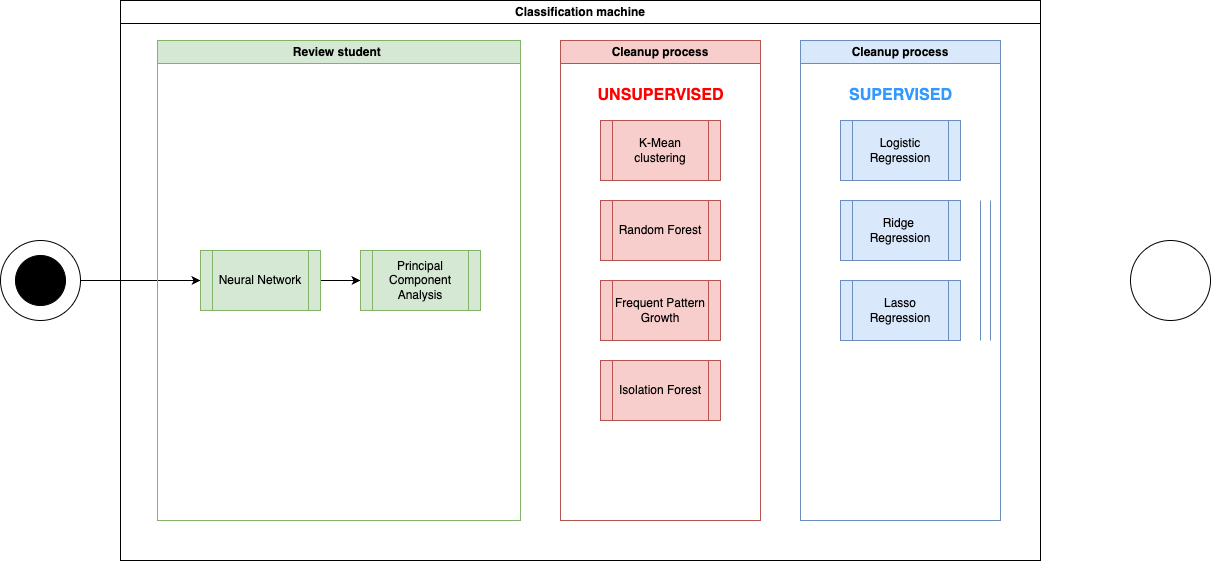
\includegraphics[width=1\linewidth]{res//diagram/ML Workflow.png}
    \caption{Algorithmic workflow for data-driven student success prediction.}
    \label{fig:dataworkflow}
\end{figure}

Each component of the workflow serves a strategic purpose:

\begin{enumerate}
    \item \acrfull{nn}: To model complex non-linear relationships and interactions among the input variables.
    \item \acrfull{pca}: For dimensionality reduction, facilitating computational efficiency and data visualization.
    \item K-Mean clustering: To identify natural groupings within the student population.
    \item Isolation Forest: For anomaly detection, highlighting atypical cases that may require special attention.
    \item Lasso Regression: To perform feature selection, enhancing model interoperability by isolating significant predictors.
\end{enumerate}

\subsection{Validation and Expected Outcomes}
We anticipate that this workflow will yield a robust model capable of identifying excellent students. We will gauge the efficiency of our model through rigorous validation techniques such as \acrfull{roc}, \acrfull{pca}, etc. to ensure the reliability of our predictions. 
To do this evaluation process, we will organize our datasets' intro training and testing sets. When training our model and test it for the first few times, we will feed it previous years' candidate profile and will examine the output of our model (i.e. potential excellence student) and compare the list given by it to the result of the entire class. This will help us determine which student could be classified as excellence and see if our model sends us back their profile or missed on some, or  to determine if our model as correctly found or missed on excellence.  
We will test our models with different year to determine if this model could be implemented and use on \textit{the field} to help institution with the registration problem.

\subsection{Usage on the field}
We would like to explain our vision on how this could be implemented in universities and institution if the model proves to be viable and efficient. Such a system would pose an ethical problem and would need to be constantly measured, evaluated and should only be administrated by a third party without interest. It would be an impartial entity without any connection with the institution. 
This model should not be used to exclude students, but should only point out the best result for each formation to reduce dropout rates throughout the country. However, other factors outside this model should be studied by administration for each institution for each formation to correctly select student not only based on the result indicated by our result but also taking into account these other factors. Moreover, any person using this model should not understand which information is used and how by the model itself. People selecting student's should not have anything to do with the registration data, the feeding process and the output of the model. To make this process as imperial as possible, this people should only receive the output without prior knowledge and the resource they usually get to chose student to do their selection.  
Finally, as said earlier in this paper to protect students, no personal information and their identity (name, surname, country of origin, etc.) should not be involved in the process and the information shared should not allow anyone to trace back the student based on the information given.That is why having compartmentalisation is really important if this system should be put in place in any institution.

\end{document}